\chapter{Design and implementation}\label{implementation}
\section{Setup at Hj{\o}rring Library}
The initial steps of the setup was to determine the location at the library where the installation would be located. The library offered a series of different locations. The chosen location is in the middle of the library. The main reason for this choice was that the area had artificial lighting and is also the most direct path from the entrance to the working area and the children's area. In figure \ref{fig:library_floorplans} the layout of the library is shown along with the designated project area.

%During the last weeks of the project, the group setup the project at Hj{\o}rring Library in order to test it and make the final arrangements. The project itself requires a canvas, some illumination from infrared LEDs, an infrared camera and a projector.

Before the actual installation a sketch of the setup was created and discussed.

The area was selected because it provides a good place for the projector and canvas. The bookshelf is a sturdy and relatively unreachable place for the projector, so no visitor will accidentally touch or mess with it.

Behind the canvas a strip of LEDs are placed. Between the projector and the canvas there is a long red bookshelf (dubbed "den r{\o}de tr{\aa}d"); this will also be used to mount a strip of infrared LEDs. In figure \ref{fig:setup_model} the setup is illustrated:

\begin{figure}[htbp] 
\centering 
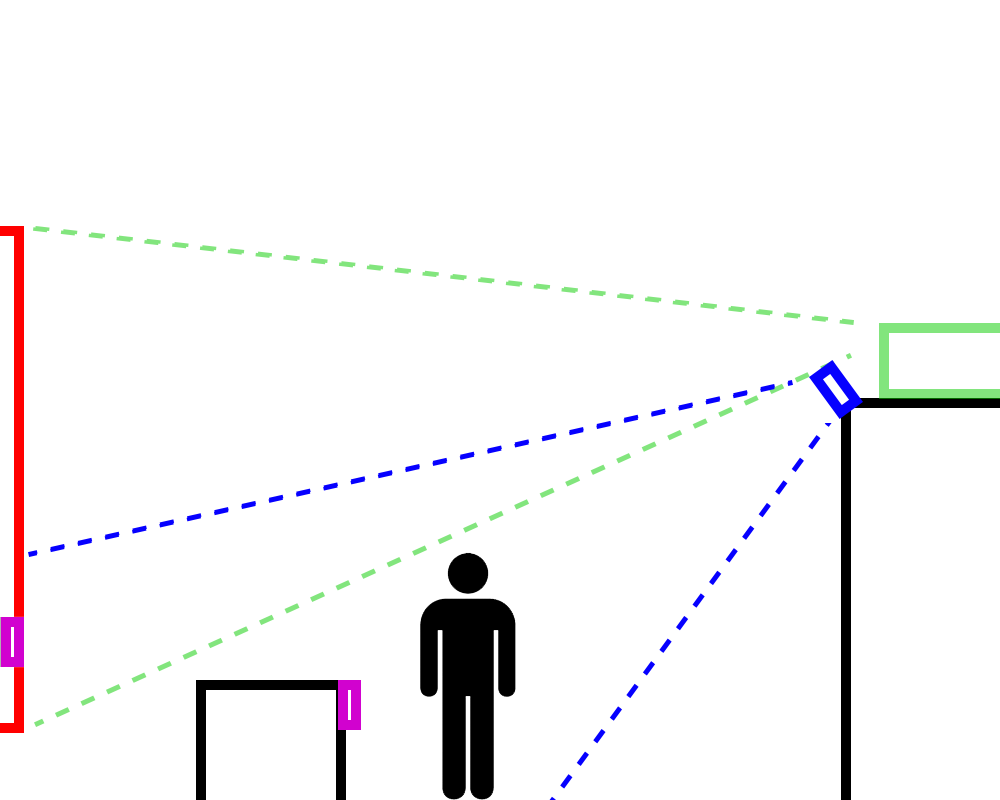
\includegraphics[width=0.8\textwidth]{Pictures/Setup/sideview_camera_with_person_two_strips.png} 
\caption{Sketch of the setup: Canvas is red; LED strips are purple; camera with IR filter is blue; projector is faded green.} 
\label{fig:setup_model} 
\end{figure}

The feasibility of the model was tested during several visits at the library. The projector's and camera's placements were tested, and proved to be suitable for implementation.

\textbf{Maybe move this to implementation about limitations and choices? - Gustav}
However, there proved to be a problem with one of the two LED strips: the strip mounted on the wall did not, due to the angle of and distance to the camera, cover the intended ROI. Therefore adjustments were made to the installation, and one row of LEDs were removed.

\subsection{LED strips}
The first step on the construction of the canvas was to position two LEDs strips in order to get the desired illumination for the infrared camera. As the placement of this project is a corridor divided by a red bookshelf that crosses the whole library, it was decided to add one strip on the lower part of this shelve and another LED stripes on the background covered by the canvas (see figure \ref{fig:LEDsPosition}).

\begin{figure}[htbp] 
\centering 
\includegraphics[width=0.8\textwidth]{Pictures/Design/stand1.png} 
\caption{Canvas placement.}
\label{fig:LEDsPosition} 
\end{figure}

The construction of these LED strips was made as simple in order to make it as light as possible. So finally the stripes were tapped to the shelves with duct tape. The solutions can be seen on figure \ref{fig:RealLEDs} and \ref{fig:RealRedLEDs}.

\begin{figure}[htbp] \centering
\begin{minipage}[b]{0.45\textwidth} \centering
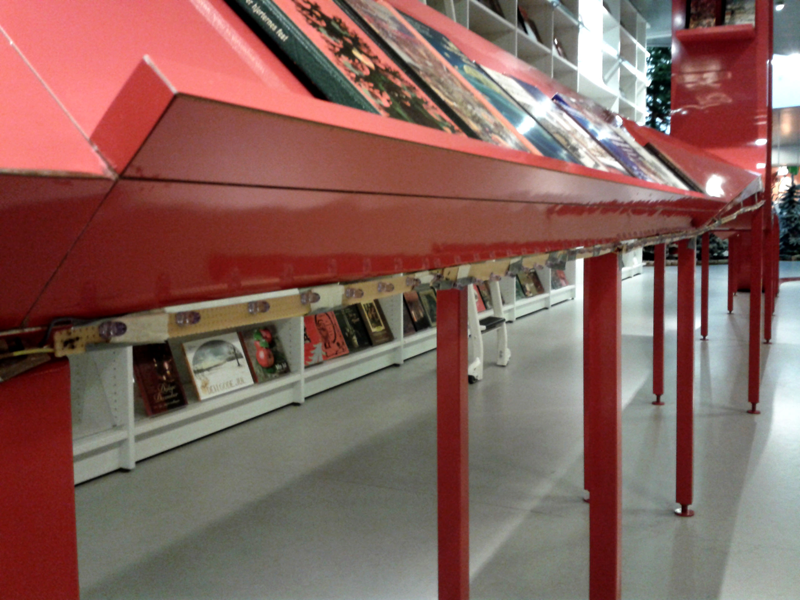
\includegraphics[width=1.00\textwidth]{Pictures/Design/LEDRedShelve.png}
\caption{LED stripes construction}
\label{fig:RealRedLEDs}
\end{minipage} \hfill
\begin{minipage}[b]{0.45\textwidth} \centering
\includegraphics[width=1.00\textwidth]{Pictures/Design/LEDShelve.png} 
\caption{LED stripes construction}
\label{fig:RealLEDs}
\end{minipage} \hfill
\end{figure}

\subsection{Building the canvas}
\textbf{Need to write more here? - Gustav}


For the projection it was decided to use a sheet to cover the bookcase behind it. Two sheets were needed to cover the area. Originally it was planned to build a custom wood box for the sheets, but due to time constraints it was instead chosen to use velcro tape to hang it up.
\begin{figure}[htbp] 
\centering 
\includegraphics[width=0.8\textwidth]{Pictures/Design/stand2.png} 
\caption{Light as captured by a camera} 
\label{fig:CanvasPosition} 
\end{figure}

